\section{Hyperspectral Image Compression}
\label{sec:compression}

The \acrfull{CCSDS} is a multi-institutional working group developing algorithms and standards for increased cooperation amongst space actors. A portion of their work has been concerned with the effective encoding of hyperspectral and multispectral images. Standard CCSDS 123.0-B-1, hereby referred to as issue 1, describes a lossless compression algorithm tailored for high throughput \acrshort{FPGA} implementations. Issue 1 has been implemented and used successfully by several missions, the \acrshort{hypso} project being one of them \cite{fjeldtvedtEfficientRealTimeFPGA2018, bakkenHYPSO1CubeSatFirst2023}. In 2019, Issue 1 was followed by standard CCSDS 123.0-B-2, referred to as Issue 2. The following sections are based on the description of issue 2 presented in \fullcite{theconsultativecommitteeforspacedatasystemsLowComplexityLosslessNearLossless2019}.

Issue 1 formalizes the \acrfull{FL} algorithm presented by \citeauthor{KlimeshFL}, which uses an adaptive filtering prediction technique to achieve lossless compression at low computational complexity suitable for space applications \cite{KlimeshFL, LosslessMultispectralHyperspectral2022}. To meet the needs of limited satellite downlink capabilities, lossy compression techniques have seen increasing use \cite{LosslessMultispectralHyperspectral2022}. For this reason, issue 2 introduces a new near-lossless feature based on the \acrfull{FLEX} algorithm presented by \citeauthor{KeymeulenFLEX} \cite{KeymeulenFLEX}. Near-lossless compression, as opposed to lossy compression, provides the user with fine-tuned control over the per-pixel loss through tunable error limit parameters.

\begin{figure}[ht]
	\begin{center}
		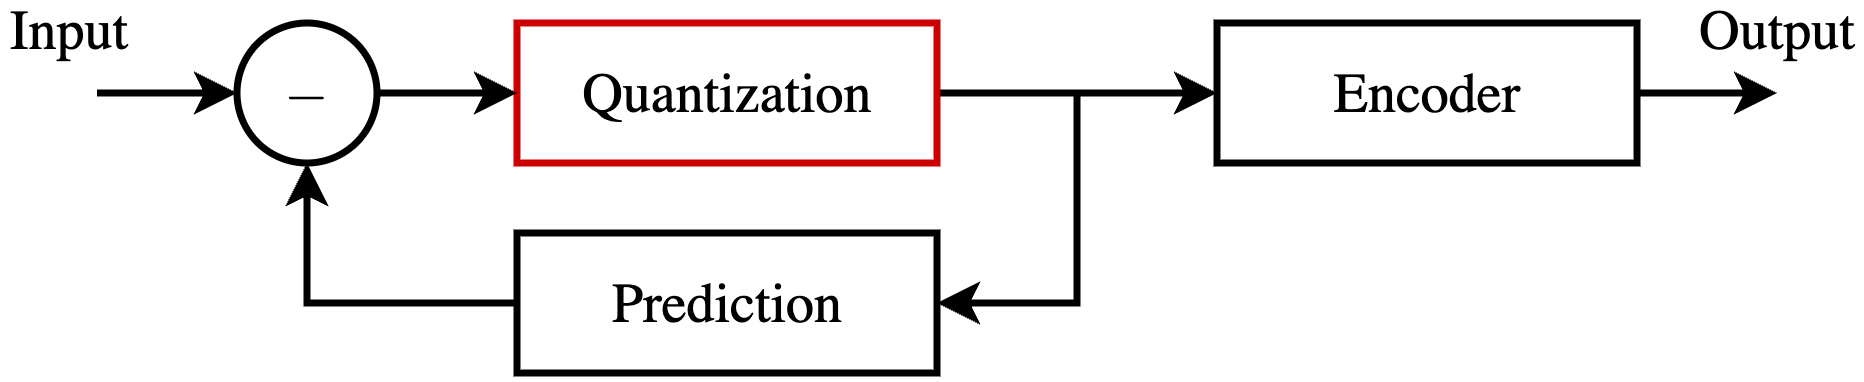
\includegraphics[width=0.7\textwidth]{figures/DPCM.png}
	\end{center}
	\caption{Layout of a differential pulse code modulator. The prediction loop, with optional quantization, reduces the entropy in the data passed to the encoder.}
	\label{fig:DPCM}
\end{figure}

The issue 1 and issue 2 compressors use a form of \acrfull{DPCM}, presented in \autoref{fig:DPCM}. A feedback loop, with optional quantization, predicts the value of the current input sample based on previously processed samples. The difference between the sample and the prediction, called the prediction residual, is encoded in the final bitstream. This exploits the correlation between neighbouring samples inherent in image data to reduce the entropy of the data passed to the encoder, allowing a more efficient encoding. Samples are processed in a single pass using simple operations. This reduces memory requirements and makes the algorithm suitable for hardware implementations. For the rest of this document, the prediction feedback loop will be referred to as the predictor.

Predictor outputs are passed to an entropy encoder which losslessly encodes prediction residuals in the final bitstream. Entropy encoders, which will be covered in greater detail later in this document, encode samples with a varying number of bits based on the frequency of their occurrence in the image. A novel feature of issue 2 is the inclusion of a hybrid encoder, in addition to the sample adaptive and block adaptive encoders of issue 1. This performs better at the low encoding bitrates achievable in the near-lossless mode. After encoding, a header containing image metadata and compressor configuration parameters is prepended to the compressed bitstream (image body). This is required by the decompressor in order to correctly reconstruct the original image.

The predictor uses an adaptive linear filter method based on the work presented by \citeauthor{gershoAdaptiveFilteringBinary1984} \cite{gershoAdaptiveFilteringBinary1984, LosslessMultispectralHyperspectral2022}. Observed quantities $x_k$, analogous to the quantized prediction residuals of \autoref{fig:DPCM}, which are statistically dependant on the process $d_k$, analogous to the image samples, produce estimates $z_k$ of the desired samples $d_k$. A linear preprocessor $\phi$ takes previously observed quantities $x_k$ and transforms them to a vector $\mathbf{u}_k$ given by

\begin{equation}
	\mathbf{u}_k = \Phi(x_k, x_{k-1}, \ldots).
	\label{eq:preprocessor}
\end{equation}

The elements of $\mathbf{u}_k$ are weighted by a vector $\mathbf{c}_k$ to produce the prediction $z_k$ as

\begin{equation}
	z_k = \mathbf{c}_k \cdot \mathbf{u}_k.
	\label{eq:predicted-value}
\end{equation}

The weight vector is adapted (updated) in increments $\Delta\mathbf{c}_k$ based on observed error residuals $z_k - d_k$ of previous predictions.

\begin{figure}[ht]
	\begin{center}
		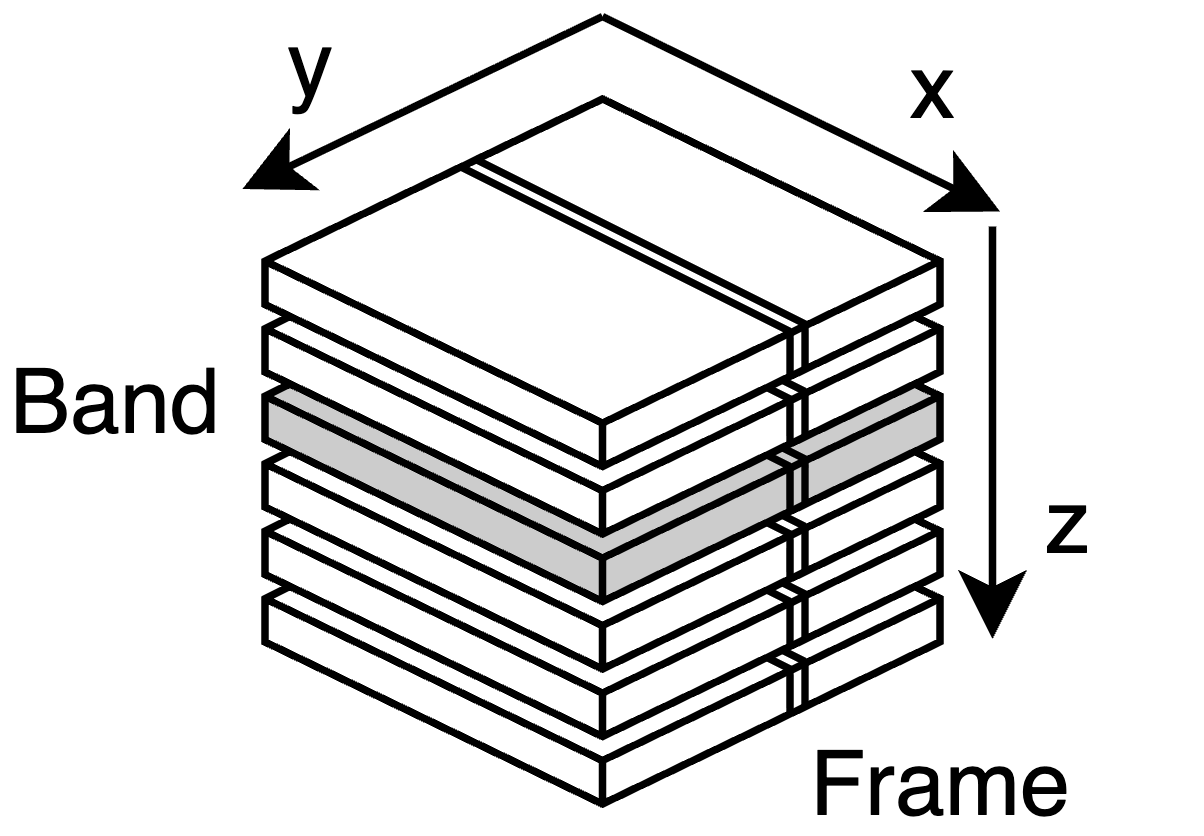
\includegraphics[width=0.3\textwidth]{figures/hsi.png}
	\end{center}
	\caption{Layout of a hyperspectral image. Samples of the same $z$ coordinates belong to the same frequency band, whereas samples of the same $y$ coordinate are denoted as frames. Samples within the same frame of a band are denoted as lines.}
	\label{fig:hsi}
\end{figure}

\autoref{fig:hsi} shows the layout of a hyperspectral image. The sizes of the dimensions $x$, $y$, and $z$ are denoted $N_x$, $N_y$, and $N_z$. Samples of the same $z$ coordinate correspond to frequency bands, while samples of the same $y$ coordinate are denoted as part of the same frame. In a bushbroom imager, like the one on-board the HYPSO-1 mission, images are captured one frame at a time \cite{grotteOceanColorHyperspectral2022}. As the satellite moves, subsequent frames are concatenated to form the final image. The camera frame rate controls the time, and thus physical space, between captured frames. Samples within the same frame of a band are referred to as lines, and samples of the same $x$ and $y$ coordinate belong to a pixel.

\begin{figure}[ht]
	\begin{center}
		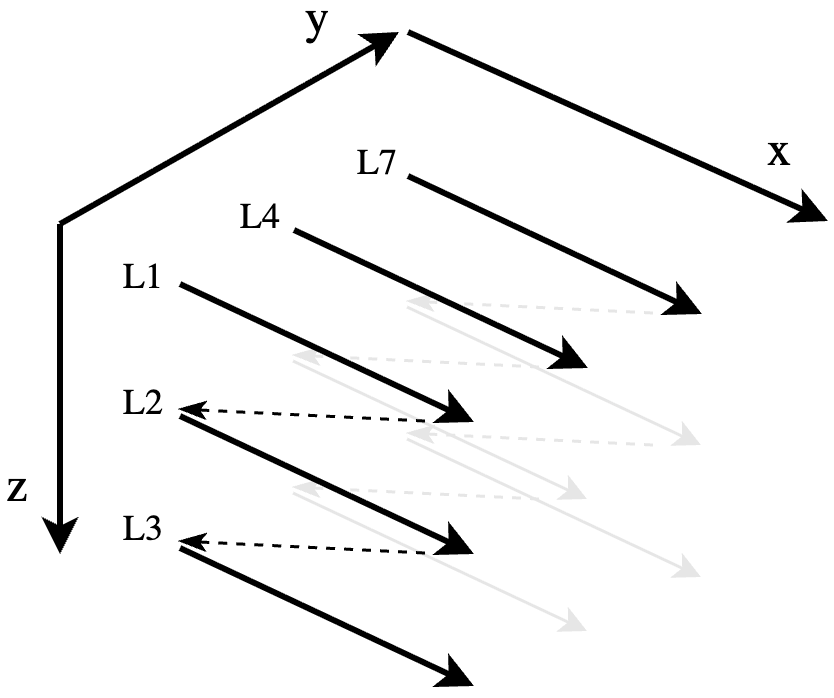
\includegraphics[width=0.3\textwidth]{figures/BIL.png}
	\end{center}
	\caption{\acrshort{BIL} processing order. Lines, L1 to L3, within the first frame are processed before proceeding to the next frame.}
	\label{fig:BIL}
\end{figure}

In order to correctly reproduce the original image, the sample processing order of the compressor and decompressor must be the same. The standard recognizes two main categories of processing orders: \acrfull{BSQ} and \acrfull{BI}. \acrshort{BSQ} ordering processes samples in coordinate order (x, y, z), meaning all samples of one band are processed before proceeding to the next. \acrshort{BI} ordering processes samples frame by frame. The frame interleaving depth $M$ dictates the processing order within the frame. The standard defines two special cases: \acrfull{BIL} and \acrfull{BIP}, with interleaving depths equal to $1$ and $N_z$ respectively. \acrshort{BIL} processes samples within a frame line by line in coordinate order (x, z, y), as presented by \autoref{fig:BIL}. \acrshort{BIP} processes samples in the order (z, x, y).

Image samples may be referred to by their $x$, $y$, and $z$ coordinates as $s(x,y,z)$. To shorten the notation, the standard introduces the spatial index $t$, given by $t = yN_x + x$. Thus, a sample may be referred to as $s_z(t)$. The number of bits used to represent a sample is the dynamic range $D$.

The following sections give a brief technical overview of the predictor and encoder stages of the issue 2 algorithm. Symbols are mentioned in text, and are the same as those used in the issue 2 standard unless otherwise is specified. As a quick reference, and for the readers convenience, all symbols are listed in \autoref{tab:compressor-symbols}. For a detailed review of the standard please see \fullcite{theconsultativecommitteeforspacedatasystemsLowComplexityLosslessNearLossless2019}.

\begin{table}[ht]
	\caption{Issue 2 compressor symbol table.}
	\label{tab:compressor-symbols}
	\begin{center}
		\begin{tabular}[c]{l|l}
			\hline
			\multicolumn{1}{l|}{\textbf{Symbol}} &
			\multicolumn{1}{l}{\textbf{Name}}                                                      \\
			\hline
			$s_z(t)$                             & Image sample                                    \\
			$\sigma_z(t)$                        & Local sum                                       \\
			$\mathbf{U}_z(t)$                    & Local difference vector                         \\
			${d}_z(t)$                           & Central local difference                        \\
			$\hat{d}_z(t)$                       & Predicted central local difference              \\
			$\breve{s}_z(t)$                     & High-resolution predicted sample                \\
			$\tilde{s}_z(t)$                     & Double-resolution predicted sample              \\
			$\hat{s}_z(t)$                       & Predicted sample                                \\
			$\Delta_z(t)$                        & Prediction residual                             \\
			$m_z(t)$                             & Maximum error                                   \\
			$q_z(t)$                             & Signed quantizer index                          \\
			$s'_z(t)$                            & Clipped quantizer bin center                    \\
			$s''_z(t)$                           & Sample representative                           \\
			$\theta_z(t)$                        & Predicted sample and sample endpoint difference \\
			$\delta_z(t)$                        & Mapped quantizer index                          \\
			$e_z(t)$                             & Double-resolution prediction error              \\
			$\mathbf{W}_z(t)$                    & Weight vector                                   \\
			$\tilde{\Sigma}_z(t)$                & High-resolution accumulator                     \\
			$\Gamma(t)$                          & Counter                                         \\
			\hline
		\end{tabular}
	\end{center}
\end{table}

\subsection{Predictor}

\begin{figure}[ht]
	\begin{center}
		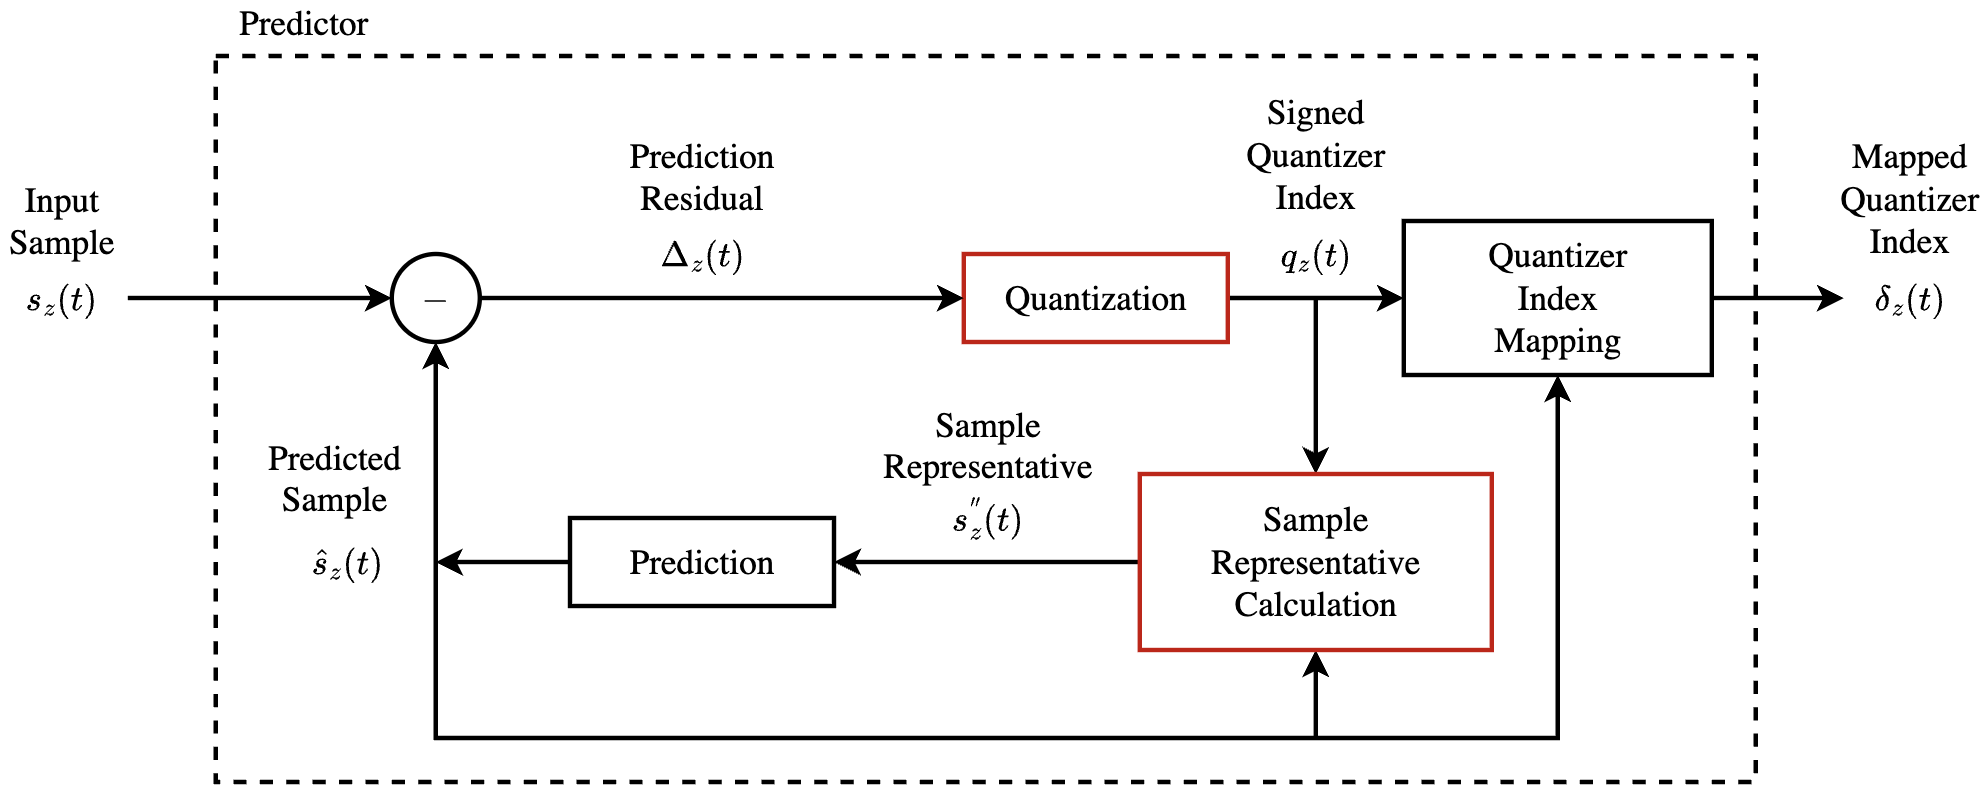
\includegraphics[width=0.9\textwidth]{figures/predictor-block.png}
	\end{center}
	\caption{Block diagram of the predictor stage of issue 2. The quantization and sample representative steps, marked in red, are new inclusions compared to Issue 1.}
	\label{fig:predictor-block}
\end{figure}

\autoref{fig:predictor-block} shows a block diagram of the issue 2 predictor stage with new features as compared to issue 1 marked in red. In the decompressor, the outputs of the predictor stage are first losslessly reproduced by decoding the encoder outputs stored in the compressed bitstream. In order to correctly retrieve the original image, the decompressor must be able to reproduce the prediction model of the compressor. Normally, this would require the samples from the original image to be known. To solve this, the issue 2 predictor makes use of sample representatives $s''_z(t)$ which may be calculated directly from the quantized prediction residuals, and thus available when decompressing.

\subsubsection{Quantization}

Prediction residuals $\Delta_z(t)$ are quantized by a uniform quantizer producing quantizer indexes $q_z(t)$ given by

\begin{equation}
	q_z(t) =
	\begin{cases}
		\Delta_z(0),                                                                                            & t = 0, \\
		\operatorname{sgn}(\Delta_z(t)) \left\lfloor \dfrac{|\Delta_z(t)| + m_z(t)}{2m_z(t) + 1} \right\rfloor, & t > 0,
	\end{cases}
	\label{eq:quantizer-index}
\end{equation}

where the prediction residual is the difference between input samples $s_z(t)$ and predicted sample values $\hat{s}_z(t)$ given by

\begin{equation}
	\Delta_z(t) = s_z(t) - \hat{s}_z(t).
	\label{eq:prediction-residual}
\end{equation}

\begin{figure}[ht]
	\begin{center}
		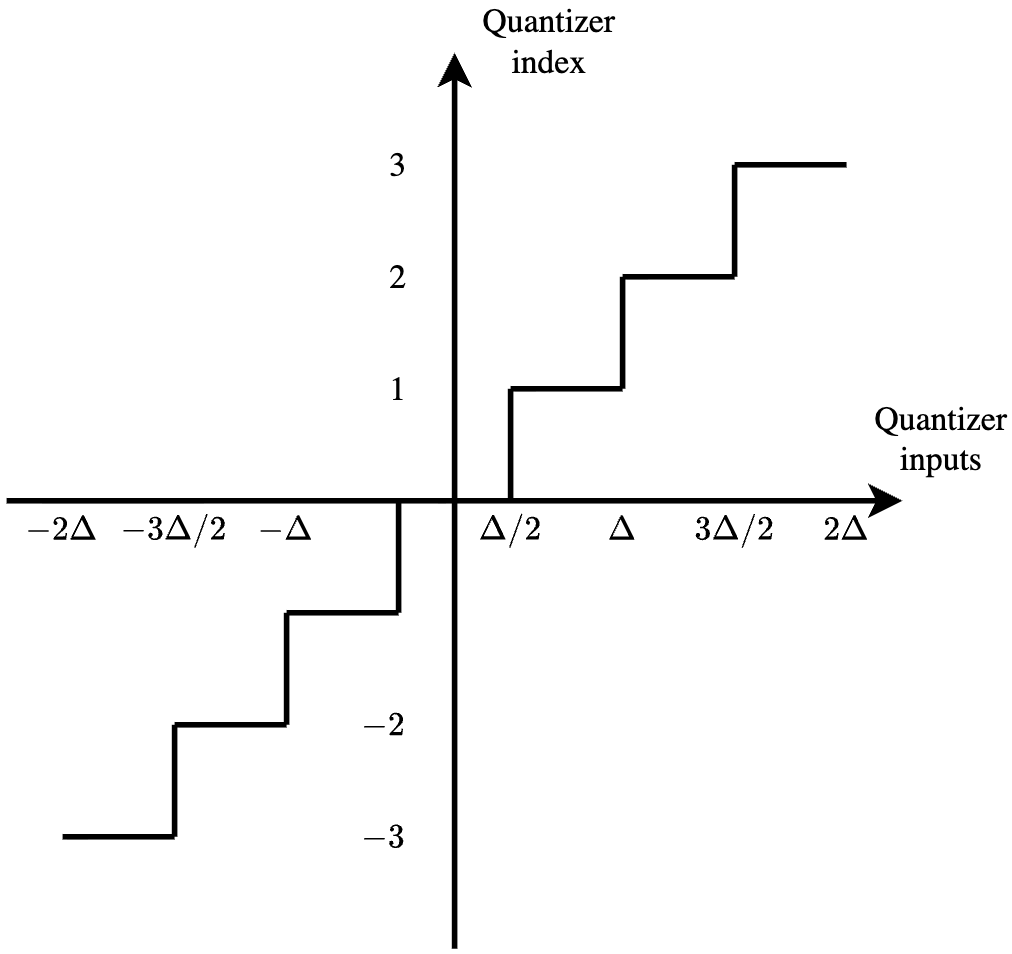
\includegraphics[width=0.5\textwidth]{figures/quantizer.png}
	\end{center}
	\caption{Uniform quantizer with step size $\Delta$.}
	\label{fig:quantizer}
\end{figure}

\autoref{fig:quantizer} shows a uniform quantizer centered at zero. Inputs are mapped to bins with size $\Delta$, also called the step size \cite{woodsDigitalImageCompression2012}. The step size of the issue 2 quantizer is $2 m_z(t) + 1$ and is controlled by the maximum error value $m_z(t)$. This guaranties that the prediction residual can be reconstructed with an error of at most $\pm m_z(t)$. A quantizer index of zero means that the predicted sample was within $m_z(T)$ of the actual sample. Positive and negative quantizer indexes indicate that the prediction overshot and undershot the sample, respectively. The clipped quantizer bin center  $s'_z(t)$ is used for calculation of sample representatives, and is given by

\begin{equation}
	s'_z(t) = \operatorname{clip}\!\left( \hat{s}_z(t) + q_z(t)\bigl(2m_z(t)+1\bigr),\ \{s_{\min},\, s_{\max}\} \right),
	\label{eq:quantizer-bin-center}
\end{equation}

where $s_{min}$ and $s_{max}$ are the lower and upper bounds for the input sample value dictated by the dynamic range $D$.

The user may select an absolute and a relative error limit, $a_z$ and $r_z$ respectively, giving fine tuned control over the per pixel difference as compared to the original image. To losslessly encode image samples, the maximum error limit may be set to zero. When error limits are used, the maximum error is given by

\begin{equation}
	m_z(t) = \min \left( a_z,\ \left\lfloor \frac{\left| r_z \,\hat{s}_z(t) \right|}{2^D} \right\rfloor \right).
	\label{eq:maximum-error}
\end{equation}

Because the codewords used by the entropy encoder to produce the compressed bitstream are only defined for positive integers, the signed quantizer indexes are mapped to positive integer mapped quantizer indexes $\delta_z(t)$. This mapping is reversible and is given by

\begin{equation}
	\delta_z(t) =
	\begin{cases}
		|q_z(t)| + \theta_z(t), & |q_z(t)| > \theta_z(t),                             \\
		2|q_z(t)|,              & 0 \le (-1)^{\tilde{s}_z(t)} q_z(t) \le \theta_z(t), \\
		2|q_z(t)| - 1,          & \text{otherwise},
	\end{cases}
	\label{eq:mqi}
\end{equation}

where the double-resolution predicted sample value $\tilde{s}_z(t)$ is an intermediate value produced by the prediction stage (\autoref{fig:predictor-block}) which will be covered later in the document. The predicted sample and sample endpoint difference $\theta_z(t)$ is given by

\begin{equation}
	\theta_z(t) =
	\begin{cases}
		\min\{\hat{s}_z(0) - s_{\min},\ s_{\max} - \hat{s}_z(0)\}, & t = 0, \\
		\min\left(
		\left\lfloor \dfrac{|\hat{s}_z(t) - s_{\min} + m_z(t)|}{2m_z(t) + 1} \right\rfloor,\
		\left\lfloor \dfrac{|s_{\max} - \hat{s}_z(t) + m_z(t)|}{2m_z(t) + 1} \right\rfloor
		\right),                                                   & t > 0.
	\end{cases}
	\label{eq:theta}
\end{equation}

\subsubsection{Sample representatives}

As mentioned, sample representatives are used in place of the sample values in order to allow the decompressor to reproduce the prediction model. Selecting sample representatives to be equal to quantizer bin center minimizes the per-pixel reconstruction error. However, a different selection may be used to minimize other quality metrics, such as the \acrfull{MSE} (\autoref{sec:metrics}) \cite{LosslessMultispectralHyperspectral2022}. For this reason, the user is provided with a set of parameters which control the selection of the sample representatives in relation to the quantizer bin center.

\subsubsection{Local Sums and Differences}

\begin{figure}[ht]
	\begin{center}
		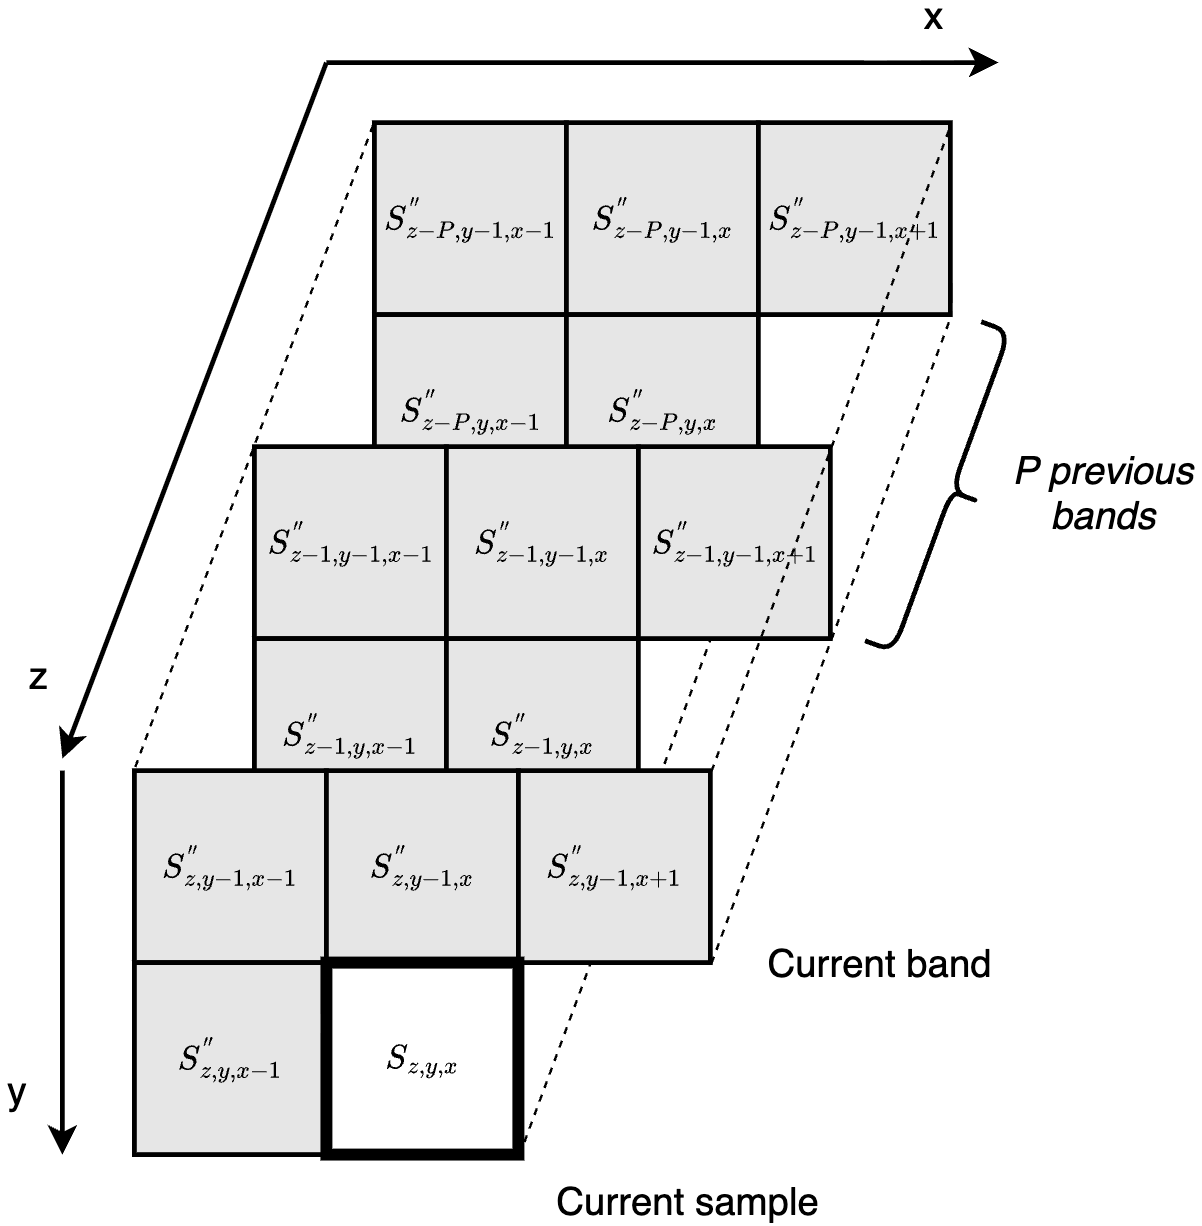
\includegraphics[width=0.7\textwidth]{figures/prediction-neighborhood.png}
	\end{center}
	\caption{A typical prediction neighborhood. Local sums are used to find local differences in $P$ previous bands (prediction bands) which are used to find the predicted sample.}
	\label{fig:prediction-neighborhood}
\end{figure}

\begin{figure}[ht]
	\begin{center}
		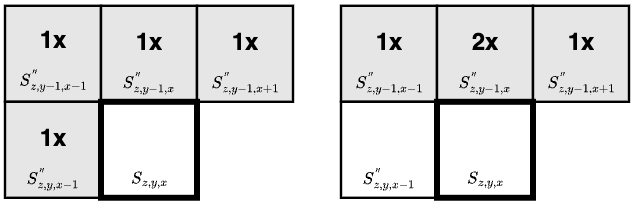
\includegraphics[width=0.7\textwidth]{figures/local-sums.png}
	\end{center}
	\caption{Wide and narrow neighbor-oriented local sum configurations.}
	\label{fig:local-sums}
\end{figure}

\begin{equation}
	\sigma_{z,y,x} =
	\begin{cases}
		s''_{z,\,y-1,\,x-1} + 2 s''_{z,\,y-1,\,x} + s''_{z,\,y-1,\,x+1},
		 & y > 0,\ 0 < x < N_X - 1,
		\\[6pt]
		4 s''_{z-1,\,y,\,x-1},
		 & y = 0,\ x > 0,\ z > 0,
		\\[6pt]
		2\!\left( s''_{z,\,y-1,\,x} + s''_{z,\,y-1,\,x+1} \right),
		 & y > 0,\ x = 0,
		\\[6pt]
		2\!\left( s''_{z,\,y-1,\,x-1} + s''_{z,\,y-1,\,x} \right),
		 & y > 0,\ x = N_X - 1,
		\\[6pt]
		4 s_{\text{mid}},
		 & y = 0,\ x = 0,\ z = 0.
	\end{cases}
	\label{eq:local-sum}
\end{equation}

\begin{equation}
	\mathbf{U}_z(t) =
	\begin{bmatrix}
		d_{z-1}(t)     \\
		d_{z-2}(t)     \\
		\vdots         \\
		d_{z-P^*_z}(t) \\
	\end{bmatrix},
	\label{eq:local-differences}
\end{equation}

\begin{equation}
	P^*_z = \min(z, P),
	\label{eq:prediction-bands}
\end{equation}

\subsubsection{Weight Updates}

\begin{equation}
	\hat{d}_z(t) = \mathbf{W}_z(t) \cdot \mathbf{U}_z(t).
	\label{eq:predicted-central-local-difference}
\end{equation}

\begin{equation}
	\mathbf{W}_z(t)=
	\begin{bmatrix}
		\omega_z^{(1)}(t) \\
		\omega_z^{(2)}(t) \\
		\vdots            \\
		\omega_z^{(P^*_z)}(t)
	\end{bmatrix},
	\label{eq:weight-vector}
\end{equation}

\begin{equation}
	\omega_z^{(1)}(1) = \frac{7}{8} 2^{\Omega}, \qquad
	\omega_z^{(i)}(1) = \left\lfloor \frac{1}{8}\, \omega_z^{(i-1)}(1) \right\rfloor,
	\quad i = 2,3,\ldots,P_z^{*},
	\label{eq:weight-init}
\end{equation}

\begin{equation}
	\omega_{\mathrm{min}} = -2^{\Omega+2}, \: \omega_{\mathrm{max}} = -2^{\Omega+2} - 1.
	\label{eq:weight-min-max}
\end{equation}

\begin{equation}
	\omega^{(i)}_{z, \text{offset}}(t) = \left\lfloor \frac{1}{2} \left(2^{-\rho(t)} \cdot d_{z-i}(t) \cdot \text{sgn}^+[e_z(t)] + 1 \right) \right\rfloor,
	\label{eq:weight-offset}
\end{equation}

\begin{equation}
	e_z(t) = 2s'_z(t) - \tilde{s}_z(t).
	\label{eq:double-resolution-prediction-error}
\end{equation}

\begin{equation}
	\rho(t) = \operatorname{clip}\!\left(
	\nu_{\min} +
	\left\lfloor \frac{t - N_x}{t_{\mathrm{inc}}} \right\rfloor,
	\{ \nu_{\min}, \nu_{\max} \}
	\right)
	+ D - \Omega,
	\label{eq:weight-update-scaling-exponent}
\end{equation}

\begin{equation}
	\omega^{(i)}_z(t + 1) = \text{clip} \left( \omega^{(i)}_z(t) + \omega^{(i)}_{z, \text{offset}}(t), \{ \omega_{min}, \omega_{max} \} \right),
	\label{eq:weight-update}
\end{equation}

\subsubsection{Prediction Calculation}

\subsubsection{Decompression}

\begin{figure}[ht]
	\begin{center}
		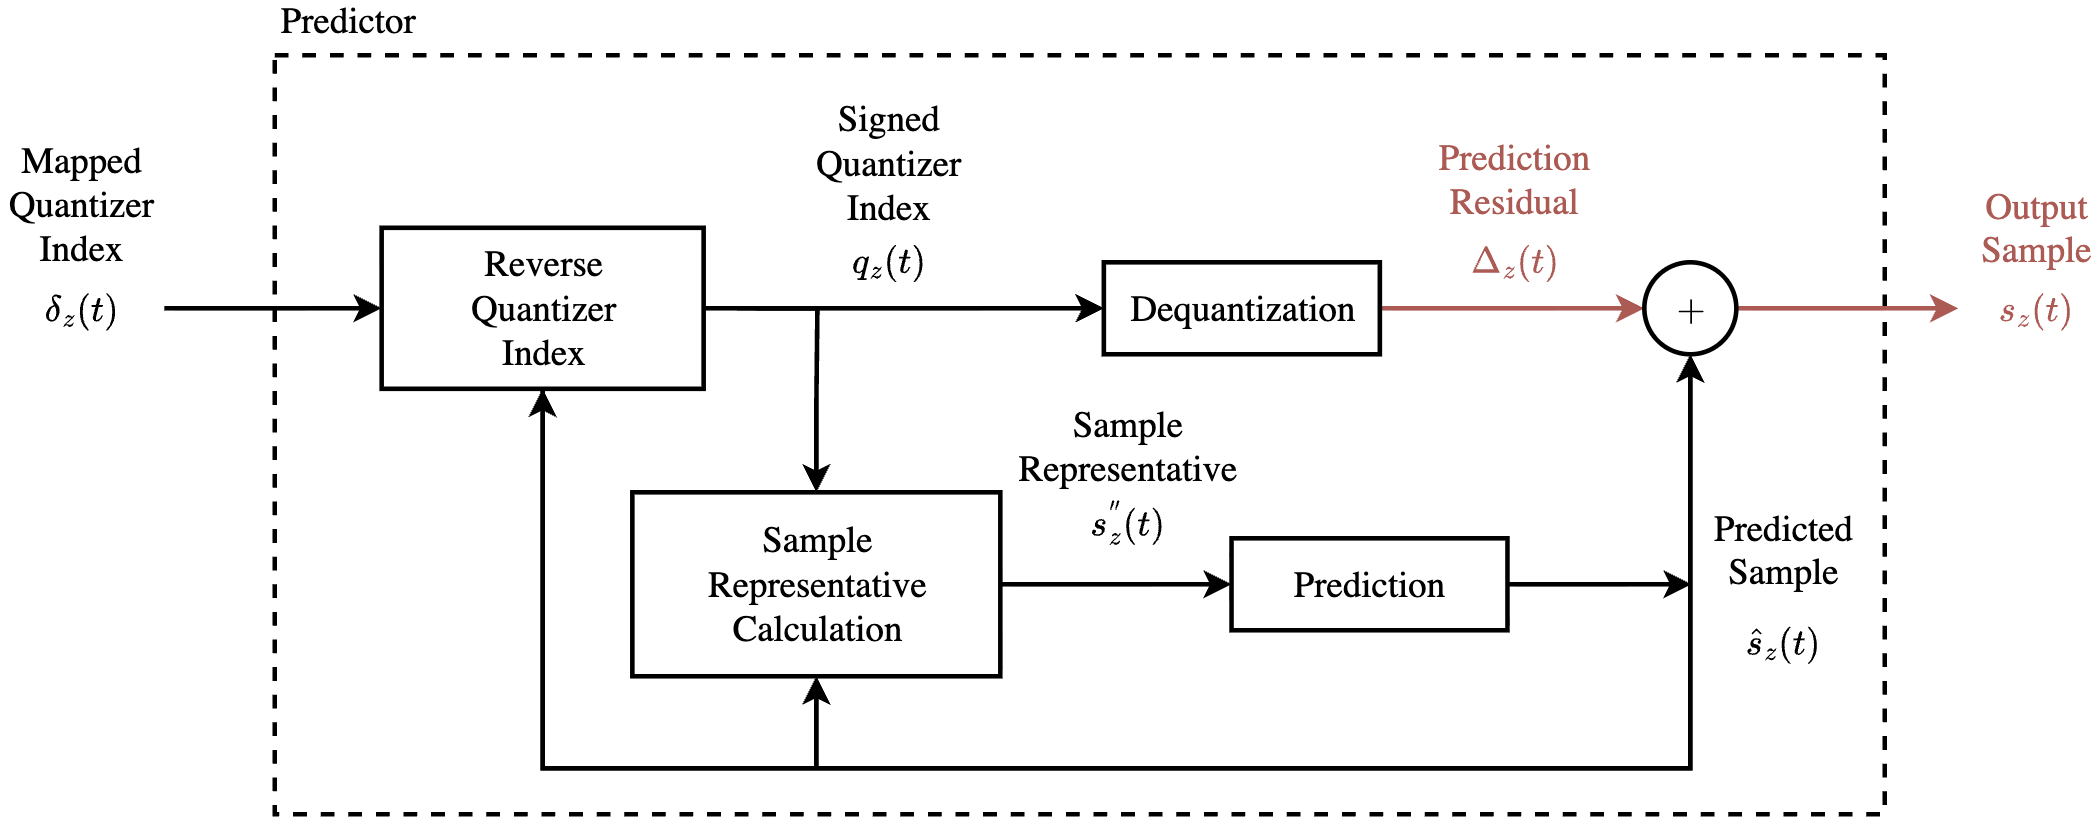
\includegraphics[width=0.9\textwidth]{figures/predictor-block-decompress.png}
	\end{center}
	\caption{Block diagram of the predictor stage of the decompressor. The prediction model is identical to that of the compressor, except for the prediction residual and reconstructed sample during near-lossless mode, marked in red.}
	\label{fig:predictor-block-decompress}
\end{figure}

Selection of quantizer bin reconstruction, center or something else...

\subsection{Header}

\subsection{Entropy Encoder}

\subsubsection{Hybrid Encoder}

\begin{equation}
	\tilde{\Sigma}_z(t) =
	\begin{cases}
		\tilde{\Sigma}_z(t-1) + 4\delta_z(t),                                           & \Gamma(t-1) < 2^{\gamma^*} - 1, \\
		\left\lfloor \dfrac{\tilde{\Sigma}_z(t-1) + 4\delta_z(t) + 1}{2} \right\rfloor, & \Gamma(t-1) = 2^{\gamma^*} - 1,
	\end{cases}
	\label{eq:accumulator}
\end{equation}

\begin{equation}
	\Gamma(t) =
	\begin{cases}
		\Gamma(t-1) + 1,                                       & \Gamma(t-1) < 2^{\gamma^*} - 1, \\
		\left\lfloor \dfrac{\Gamma(t-1) + 1}{2} \right\rfloor, & \Gamma(t-1) = 2^{\gamma^*} - 1,
	\end{cases}
	\label{eq:counter}
\end{equation}

\subsubsection{Decoding}
